\documentclass[10pt]{article}

\usepackage{fullpage}
\usepackage[margin=2cm]{geometry}
\usepackage[pdftex]{graphicx}
\usepackage{float}

\begin{document}

\title{\vspace{-2cm}ARM11 Checkpoint Report}
\author{\small Alexander CLARKE, Qiang FENG, Jordan SPOONER, Laurence SQUIRES}

\maketitle

\section{Group Organisation}

Our group would split up the work by first coming together to work out what structure our project should have. We would then work out all of the data types that we would need to implement our design for the structure and firstly implement them. After this point we may add more data types later if we realise we need more.

Using our data-types and structure we know what functions should take what data type, and what data type they should output. Our group created a shared google docs spreadsheet to track all of the functions we thought we needed to implement. There were three jobs for each function, being complete the code, create unit tests for the code and sign off the code. These jobs would be assigned to different team members, but we would sometimes do other peoples jobs if it improved our groups work flow. We would then separately implement these functions, often in separate files to make version control easier. This work flow allowed for improved parallel coding.

After creating the functions we would come together as a group to debug our program. As different people created different functions debugging as a team made it easier as we could step through each function with the person who made that code block. Once we pass all of the given tests we would check which edge cases are not tested by the given tests. We would then create our own tests to check for these edge cases.

Throughout the project we are following a style guide to ensure consistency and implementing Javadoc style comments, which allows us to automatically generate documentation with Doxygen. These resources can both be found in the \texttt{/doc} folder.

Our group is working really well together. We help each other whenever we are unsure with the specification or any other problems, and we get along really well. I don’t believe many (if any) changes would be required to do the later tasks. This is evidenced by the fact that our emulator is fully functioning and our assembler passes the majority of the test-cases. We plan for our assembler to pass all test cases by the end of today (Friday).

An adjustment that we could make is more regimented meet up times. While we all spend a long time in labs, some of us do arrive a few hours earlier. While this is an adjustment we could make it is not necessary as whenever someone arrives earlier they can begin to implement necessary functions while waiting for the rest of the team. We are already thinking up ideas for our extension, but we haven't yet determined upon a singular idea.

\begin{figure}[H]
\begin{minipage}{0.6\linewidth}

\section{Implementation Strategies}

\subsection{Implementation of \texttt{emulate.c}}

We structured our emulator as follows:

\begin{itemize}
\item \texttt{emulate.c} contains the function \texttt{main}, which takes a single parameter of the filename containing ARM11 object code. \texttt{main} calls the function \texttt{load\_file} from \texttt{toolbox.h} to load the file into memory, \texttt{decode\_instruction} and \texttt{execute} from \texttt{decode.h} and \texttt{execute.h} respectively, for the main fetch-decode-execute cycle, and \texttt{print\_system\_state\_compliant} from \texttt{print\_compliant.h}, which prints the registers and non-zeroed memory in a format which passes the automated tests.
\item \texttt{unit\_tests.c} contains a suite of simple tests that check the functionality of each of the called functions. Rather than using a unit testing framework, we opted for a simple macro and use of \texttt{assert.h} to check our functions work as documented.
\item \texttt{print\_compliant.c} contains functions for printing output to \texttt{stdout} in a way that passes test cases. It defines \texttt{print\_system\_state\_compliant} as well as several helper functions.
\end{itemize}

\end{minipage}
\hspace{0.05\linewidth}
\begin{minipage}{0.35\linewidth}

\centering
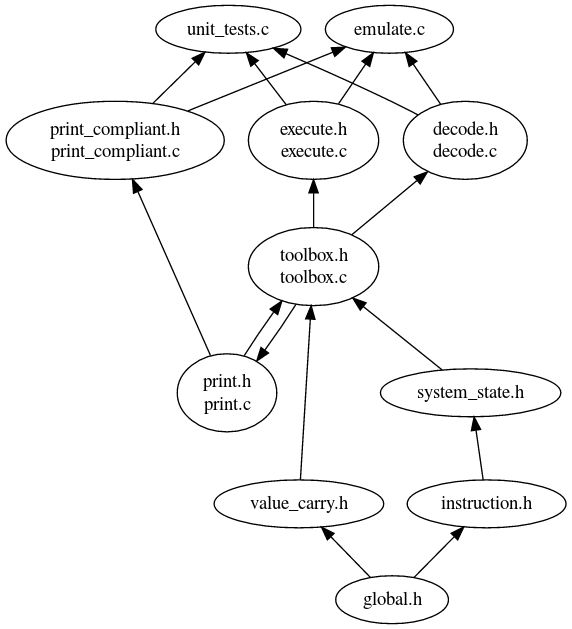
\includegraphics[scale=0.28]{Checkpoint/emulate.png}
\caption{Dependency Graph for \texttt{emulate.c}}

\end{minipage}
\end{figure}

\begin{itemize}
\item \texttt{print.c} contains functions for printing output that is extremely helpful for debugging. Some of these functions are also called by the compliant printing functions. Setting \texttt{COMPLIANT\_MODE} to \texttt{false} in \texttt{global.h} uses these functions instead of the compliant ones. The output no longer passes tests, but more details, such as the most recently fetched and decoded instructions, will be printed.
\item \texttt{decode.c} contains the function \texttt{decode\_instruction} and helper functions to decode each type (data processing, multiply, single data transfer, branch) of instruction.
\item \texttt{execute.c} contains the function \texttt{execute} and helper functions for each type of instruction.
\item \texttt{toolbox.c} contains a number of useful helper functions used throughout the code. It includes the function \texttt{load\_file}, as well as \texttt{exit\_program}, which prints the current system state before exiting cleanly, functions to read and write to memory (\texttt{get\_word} and \texttt{set\_word} respectively), functions for working with two's complement numbers, and the \texttt{shifter} function, which emulates a shifter. \texttt{get\_word} and \texttt{set\_word} already implement the requirements of Part III, by printing to \texttt{stdout} each time the GPIO pins are accessed, set or cleared.
\end{itemize}

We then have headers for each \texttt{.c} file, as well as the following headers, which are used to define constants and type aliases:

\begin{itemize}
\item \texttt{global.h}, which defines constants such as the word size, the number of registers, and the number of memory addresses, as well as the following type aliases: \texttt{byte\_t}, \texttt{address\_t}, \texttt{reg\_address\_t} and \texttt{word\_t}, which are aliases for differently sized numbers, and which make function definitions much clearer. It also defines the enumerations \texttt{condition\_t}, \texttt{instruction\_type\_t}, \texttt{opcode\_t} and \texttt{cpsr\_flags\_t}, whose functionality is clear from their type aliases.
\item \texttt{system\_state.h}, which contains the \texttt{system\_state\_t} struct, which specifies all of the information required to determine the exact state of an ARM11 machine. Specifically, it contains the contents of all registers and memory locations, the last fetched instruction, and the last decoded instruction.
\item \texttt{instruction.h}, which contains the \texttt{instruction\_t} struct, which can define a decoded instruction. It specifies the instruction type and the condition, as well as the register numbers (of which there can be a maximum of 4), an opcode (if necessary), an immediate offset or operand (if necessary), a shift type and amount (if necessary), and any other relevant bits (of which there can be a maximum of 4).
\item \texttt{value\_carry.h}, which contains an extremely simple struct \texttt{value\_carry.h}, which is used by the shifter to output a value and a carry.
\end{itemize}

For further details on the implementation, see the full documentation, which is on the GitLab repository and located at \texttt{doc/LaTeX Documentation/refman.pdf}.

\subsection{Implementation of \texttt{assemble.c}}

\texttt{assemble.c} can reuse several parts of the emulator code. Many of the constants, enums, structs, and other type aliases can be reused, saving a lot of planning time to design effective data structures. In particular, we reuse the constants and types in \texttt{global.h}, the printing functions in \texttt{print.h} (for debugging) and the \texttt{instruction\_t} struct from \texttt{instruction.h}.

Again, we have a \texttt{main} function in \texttt{assemble.c}, which calls helper functions throughout several other files, each themselves calling further helper functions. This is to allow us to each write different functions on seperate files, making version control really simple.

\subsection{Further Challenges and Implementation of the Extension}

It is difficult to say what tasks we will find difficult later on when we are not yet sure what our extension will be. I'm sure that we will find some of the tasks in our extension challenging (otherwise we have not chose a good enough extension), but at this point we do not know what they will be. For this reason, we are planning to finish Parts I to III by the beginning of next week, giving us plenty of time to work on the extension.

One of the more difficult parts of the assembler was creating a function to split up each line into a useful list of strings that could be used for other functions to much easier parse through. While creating that function can be done in an easier way, it would not be correct for the optional shift by a register. However, we have already implemented this function and it is correct for all of the given test cases. The other tasks in the assembler should be far easier in comparison.

\end{document}
